\section{Multiplanární rekonstrukce}
Po předvedení programu v IKEM byl vznesen další požadavek na funkčnost programu a to implementace multiplanární rekonstrukce (MPR).

Multiplanární rekonstrukce je specifický způsob zobrazení snímku: Obrazovka je rozdělena na tři části. V každé části vidíme řez třírozměrného snímku a to ve třech na sebe kolmých rovinách. V každém z řezů dále vidíme vyznačené průsečiky se zbylými dvěma rovinami. Lépe je vše vidět z následujícího obrázku:

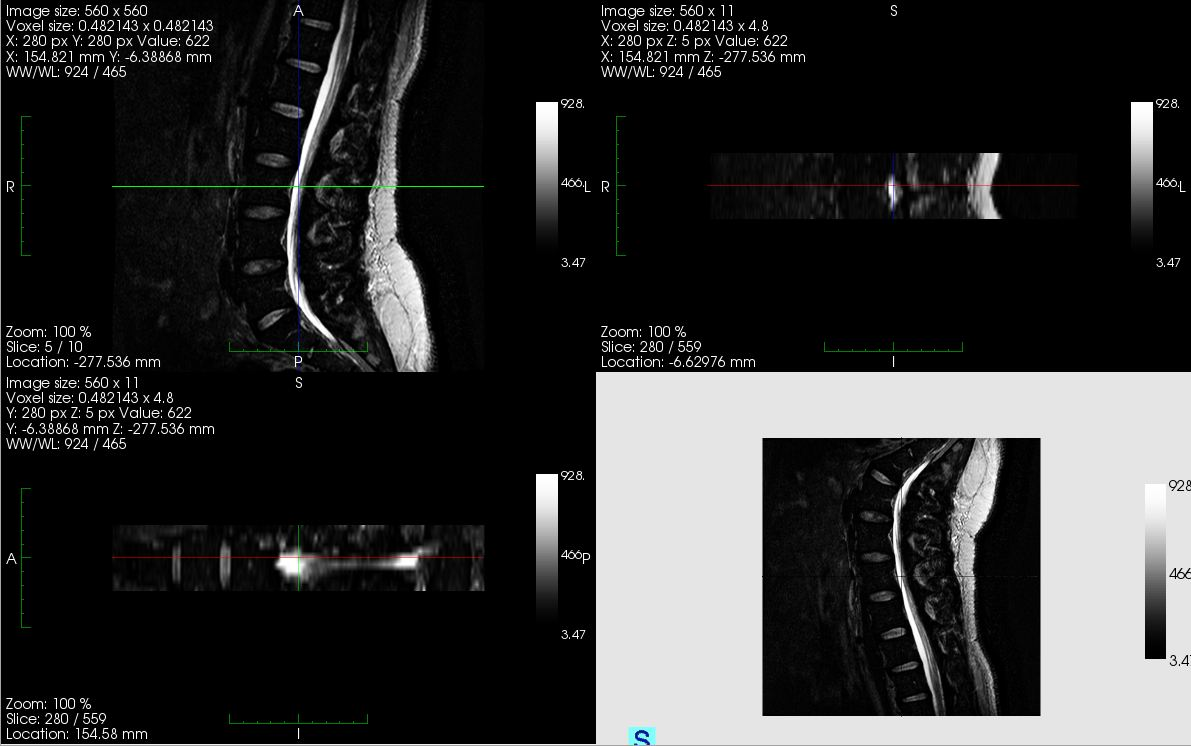
\includegraphics[width=0.9\textwidth,height=0.9\textwidth]{Text/IMG/MPR_Medinria.jpg}

\subsection{Objektový návrh Dicom-Presenteru}
Zadání bylo do stávajícího programu přidat podporu multiplanární rekonstrukce. Jelikož přidání MPR znamená zásah do stávajícího objektového návrhu programu, je nutné se nejprve stručně seznámit se stávajícím objektovým návrhem programu.

V programu DicomPresenter je vykreslování snímků na obrazovku realizováno kooperací několika různých tříd. V první řadě je možné vidět třídu, která zajišťuje zobrazení jednotlivých snímků, manipulaci se snímky uživatelem - tato třída se nazývá Workspace, neboli pracovní plocha. Program DicomPresenter umožňuje mít takovýchto pracovních ploch otevřeno hned několik a tak byly vytvořeny dvě další třídy. Jedna se stará o uložení pracovních tříd v paměti počítače - WorkspaceManager. Druhá třída je pak potřeba k přepínání mezi pracovnímí plochami uživatelem.

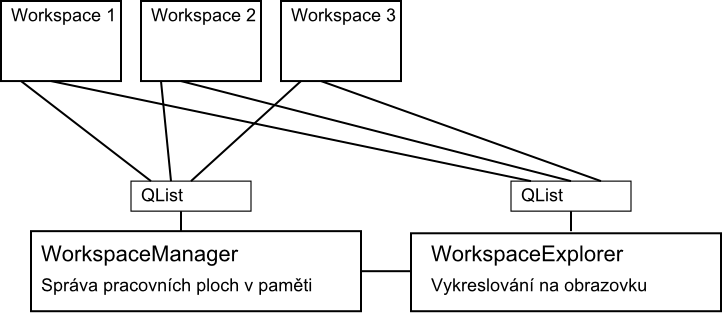
\includegraphics[width=0.9\textwidth]{Text/IMG/WorkspaceManager.png}

Do tohoto modelu je nutné někam zařadit novou třídu, která zajistí funkčnost multiplanární rekonstrukce. Byla tedy vytvořena nová třída podobná třídě Workspace, která nebude zobrazovat několik různých Dicom snímků, ale bude zobrazovat vždy jen jeden Dicom snímek v různých řezech. Bylo nutné zaručit, aby se uživatel mohl přepínat mezi novou pracovní plochou s multiplanární rekonstrukcí a mezi všemi starými pracovními plochami.

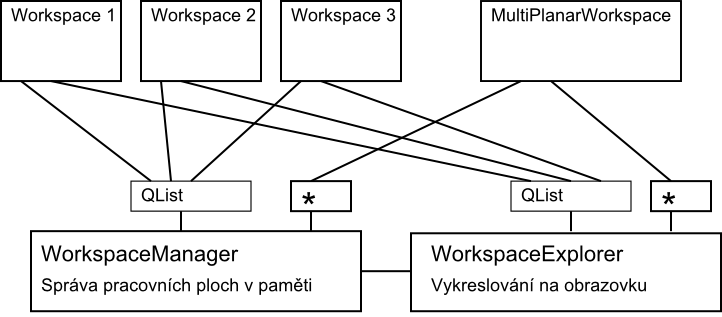
\includegraphics[width=0.9\textwidth]{Text/IMG/MultiPlanar.png}


\begin{comment}
Základním pojmen v objektovém návrhu DP je pracovní plocha (třída Workspace). Multiplanární rekonstrukce bude zobrazena na takové pracovní ploše. V této stati popíšeme třídy, jež úzce souvisí s pracovními plochami.

Pracovní plocha je reprezentována třídou Workspace. Třída Workspace se stará především o správu snímků s nimiž uživatel manipuluje a pak jejich vykreslení na obrazovku.

Třída WorkspaceManager se pak stará o uložení snímků v paměti programu. Třída vlastní objekt Qt knihovny QList, což je seznam, ve kterém jsou uloženy ukazatele na otevřené pracovní plochy.

Třída WorkspaceExplorer je pak třídou, která má na starosti grafické rozhraní, to znamená, že zajišťuje uživateli možnost manipulace s pracovními plochami: jejich otevírání, zavírání, přepínaní se mezi nimi.

Původní koncept, jak přidat do programu nový tip pracovní plochy, jež bude umožňovat multiplanární rekonstrukci byl takový, že rozdělíme třídu Workspace na dvě třídy. Více abstraktní funcke společné stávající pracovní ploše a nové pracovní ploše s MPR by pak mohly být odděleny v abstraktní třídě (nazvěme ji pro přehlednost MetaWorkspace). Tyto abstraktní funkce společné pro oba typy pracovních ploch jsou např.: vytváření animací, změna velikosti pracovní plochy, vykreslování obsahu pracovní plochy do frame bufferu atd.

Bohužel se ukázalo, že nový typ pracovní plochy bude od původní dosti odlišný ve funkčnosti, takže bylo vhodnější  vytvořit zcela odlišný typ pracovní plochy.

Pro multiplanární rekonstrukci tedy byl vytvořen nový typ pracovní plochy: třída PlanarWorkspace. Nová třída je v zásadě odlišná od původních pracovních ploch. Původní pracovní plochy obsahovali funkce pro přídávání jednotlivých snímků na obrazovku, pro přeskupování snímků atd. Všechny tyto funkce budou v pracovní ploše pro multiplanární rekonstrukci nepotřebné.

\end{comment}

\subsection{Implementace multiplanární rekonstrukce v třídě Image}
Multiplanární rekonstrukce je implementována tak, že v třídě Image byly vytvořeny nové funkce pro vykreslení tří na sebe kolmých řezů z trojrozměrné textury. Funkcím, jsou vždy předány souřadnice společného průsečíku tři dvourozměrných ploch, které zobrazujeme.

\begin{lstlisting}[label=DicomImageClass,caption={První část souboru \texttt{Window.cpp} se zdrojovým kódem třídy reprezentující okno programu.}]
void CGLImage::DrawToTextureSliceZ(TPlanarCrossPosition crossposition){
	glBindFramebufferEXT(GL_FRAMEBUFFER_EXT, iFBOZ);

 	glEnable(GL_TEXTURE_3D);
	glBindTexture( GL_TEXTURE_3D, iTexture->GetTextureID ());

	glEnable(GL_TEXTURE_2D);
	glBindTexture(GL_TEXTURE_2D, iSliceZ);

	glBegin(GL_QUADS);
	glColor4f( 1., 0., 0., 1.);
	glTexCoord3d(0,1,crossposition.z); 	glVertex2d(0,0);
	glTexCoord3d(1,1,crossposition.z); 	glVertex2d(1,0);
	glTexCoord3d(1,0,crossposition.z); 	glVertex2d(1,1);
	glTexCoord3d(0,0,crossposition.z);	glVertex2d(0,1);
	glEnd();

	glBindTexture(GL_TEXTURE_2D, 0);
	glDisable(GL_TEXTURE_2D);

	glBindTexture( GL_TEXTURE_3D, 0);
	glDisable(GL_TEXTURE_3D);

	glBindFramebufferEXT(GL_FRAMEBUFFER_EXT, 0);
}
\end{lstlisting}

Jak vidíme ve výpisu kódu, řez je pořizován z třírozměrné textury (řádky 12-15) a je kreslen do FrameBufferu (aktivace frame bufferu ř. 2), respektive pak do dvojrozměrné textury (aktivace textury ř. 7,8), která je uložena v paměti OpenGL. Z této textury je pak řez překreslen na obrazovku:

\begin{lstlisting}[label=DicomImageClass,caption={První část souboru \texttt{Window.cpp} se zdrojovým kódem třídy reprezentující okno programu.}]
void CGLImage::DrawSliceZ(){
	glEnable( GL_TEXTURE_2D );
	glBindTexture(GL_TEXTURE_2D, iSliceZ);
	glBegin( GL_QUADS );
	glTexCoord2d(0,0); 	glVertex2d(0,0.5);
	glTexCoord2d(1,0);		glVertex2d(0.5,0.5);
	glTexCoord2d(1,1);		glVertex2d(0.5,1);
	glTexCoord2d(0,1);		glVertex2d(0,1);
	glEnd();
	glBindTexture(GL_TEXTURE_2D, 0);
	glDisable(GL_TEXTURE_2D);
}
\end{lstlisting}

Změna v tom, z jaké části snímku bude pořizován aktuální řez je prováděna na základě uživatelských akcí, je tedy popsána a počítána ve funkcích Qt knihovny: mousePressEvent, mouseMoveEvent. Zajímavostí je, že PlanarWorkspace je objekt v hiearchii Qt podřazený objektu QWidget, který odpovídá hlavnímu oknu aplikace. Tedy všechny uživatelské akce zachycuje QWidget, který je pak předává podřazeným objektům.

V třídě PlanarWorkspace bylo tedy nutné definovat funkce mousePressEvent a mouseMoveEvent. Úkolem je toto: když uživatel klikne na jeden ze tří řezů, zapamatujme si pozici kurzoru. Když uživatel pohne myší v jednom ze směrů, tak podle toho přepočítejme pozici odpovídajícího řezu.

Ve funkci mousePressEvent tedy zjistíme na který z řezů uživatel klikl a zapamatujeme si pozici myši:

\begin{lstlisting}[label=DicomImageClass,caption={První část souboru \texttt{Window.cpp} se zdrojovým kódem třídy reprezentující okno programu.}]
void CGLPlanarWorkspace::mousePressEvent(QMouseEvent *event){
	int thisSizeX = this->GetSize().x();
	int thisSizeY = this->GetSize().y();
	int mousePositionX = event->x();
	int mousePositionY = event->y();
	if((mousePositionX<thisSizeX/2)&&(mousePositionY<thisSizeY/2)){
		UserManipulatingSlice = 'z';
		CGLWidget::GetInstance()->setCursor(QCursor(Qt::BlankCursor));
		iEventHistory->setX(mousePositionX);	
		iEventHistory->setY(mousePositionY);
		*iCursorHistory = QCursor::pos();
	}
	if((mousePositionX>thisSizeX/2)&&(mousePositionY<thisSizeY/2)){
 		...
	}
	if((mousePositionX<thisSizeX/2)&&(mousePositionY>thisSizeY/2)){
 		...	
	}
}
\end{lstlisting}

Na výpisu kódu je vidět, že si pozici dokonce zapisujeme dvakrát. To je zajímavý jev. Pozici kurzoru myši totiž lze počítat v absolutních hodnotách vzhledem k obrazovce počítače, nebo také v relativních hodnotách vzhledem k oknu aplikace. Pro výpočet do jakého ze tří oken s řezem textury uživatel klikl je výrazně přehlednější používat relativní souřadnice vzhledem k oknu aplikace (vyhneme se tak složitým přepočtům, když uživatel přemístí okno jinam, nebo dokonce na jiný monitor). Pokud ale chceme kurzor myši umístit po akci uživatele zpět na původní místo, což zde využíváme, je nutné tuto novou pozici zadávat v absolutních souřadnících vzhledem k obrazovce.

V těle funkce mouseMoveEvent pak počítáme o kolik uživatel pohl myší, myš vracíme na původní místo a dále nastavujeme nové souřadnice řezů. Dále je potřeba ošetřit situaci, kdy uživatel nastavuje souřadnice poblíž přípustné hranice. Na konci pak voláme překreslení OpenGL, aby se změny promítli na obrazovce.

\begin{lstlisting}[label=DicomImageClass,caption={První část souboru \texttt{Window.cpp} se zdrojovým kódem třídy reprezentující okno programu.}]
void CGLPlanarWorkspace::mouseMoveEvent(QMouseEvent *event){
	int mouseAfterMovePositionX = event->x();
	int mouseAfterMovePositionY = event->y();
	QCursor::setPos(*iCursorHistory);
	if(UserManipulatingSlice == 'z'){
		int dx = mouseAfterMovePositionX - iEventHistory->x();
		int dy = iEventHistory->y() - mouseAfterMovePositionY;
		if ((iPlanarCrossPosition.x+(float)dx/(float)iSensitivity>0.) && (iPlanarCrossPosition.x+(float)dx/(float)iSensitivity<1.))
			iPlanarCrossPosition.x=iPlanarCrossPosition.x+(float)dx/(float)iSensitivity;
		if ((iPlanarCrossPosition.y+(float)dy/(float)iSensitivity>0.) && (iPlanarCrossPosition.y+(float)dy/(float)iSensitivity<1.))
			iPlanarCrossPosition.y=iPlanarCrossPosition.y+(float)dy/(float)iSensitivity;
	}
	if(UserManipulatingSlice == 'x'){
 		...
	}
	if(UserManipulatingSlice == 'y'){
 		...
	}
	CGLWidget::GetInstance()->updateGL();
}
\end{lstlisting}

